
\subsection*{Què és la banca online?}
\addcontentsline{toc}{subsection}{Què és la banca online?}


\textbf{Banca online} és una nova modalitat d'activitats financeres que permet a les persones adscrites a un banc gestionar, mitjançant internet i mitjançant qualsevol dispositiu electrònic, la majoria de les operacions bancàries a qualsevol hora i des de qualsevol lloc. A diferència de la banca tradicional, dóna la possibilitat als clients d'una entitat d'aquestes característiques d'accedir als comptes i de realitzar múltiples procediments bancaris sense l'estricta necessitat d'una sucursal física. 


\subsection*{La primera banca online i evolució}
\addcontentsline{toc}{subsection}{La primera banca online i evolució}

La banca online es remunta a les darreres dècades del segle XX. En la dècada de 1980, els primers experiments amb serveis financers en línia van començar a aparèixer. No obstant això, en aquesta etapa, la tecnologia i la connectivitat limitades van restringir la seva adopció massiva. Posteriorment amb l'augment de la disponibilitat d'Internet i el desenvolupament de tecnologies de seguretat, els bancs van començar a oferir serveis en línia. \textbf{Wells Fargo va ser un dels primers bancs a oferir serveis bancaris en línia el 1995.}

Ràpidament el consorci de targetes de crèdit Visa i MasterCard va llançar el protocol Secure Electronic Transactions (SET) per proporcionar una capa de seguretat addicional a les transaccions en línia. A mesura que Internet es feia més accessible, la banca en línia es va expandir globalment, nombrosos bancs arreu del món van començar a oferir serveis en línia per millorar la comoditat dels seus clients. Més tard, La banca online va evolucionar amb característiques més avançades, com la capacitat de realitzar transferències electròniques, pagar factures en línia i accedir a estats de compte electrònics. Els bancs també van introduir mesures de seguretat millorades, com l'autenticació de doble factor. Actualment els bancs van desenvolupar aplicacions mòbils que permetien als usuaris realitzar transaccions bancàries des dels seus dispositius mòbils, i  continuat evolucionant amb tecnologies emergents com la intel·ligència artificial, l'aprenentatge automàtic i la blockchain. A més, la ciberseguretat s'ha convertit en una prioritat encara més gran per protegir la informació financera dels usuaris.


\begin{figure}[h]
    \centering
    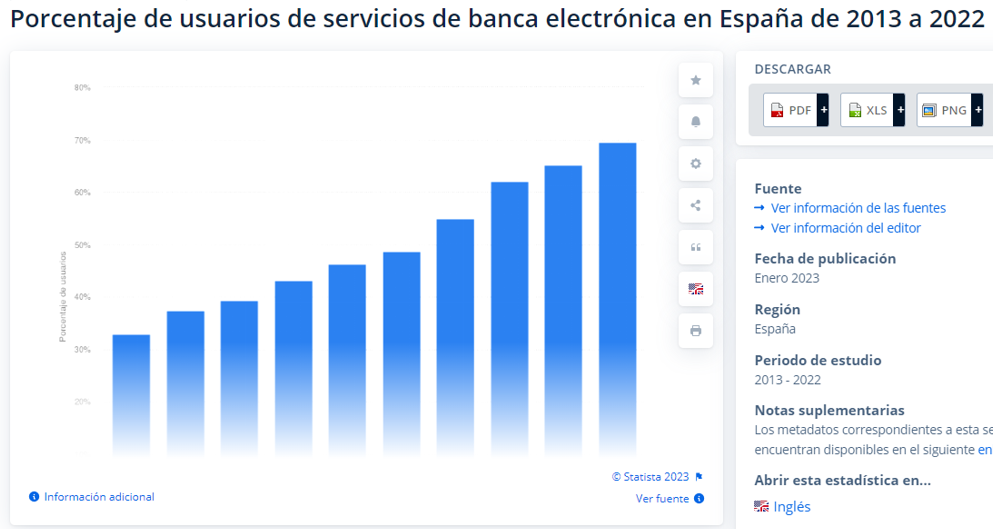
\includegraphics[width=0.6\textwidth]{percentatge.png}
\end{figure}
  


\subsection*{Les característiques principals de la banca en línia}
\addcontentsline{toc}{subsection}{Les característiques principals de la banca en línia}

La \textbf{banca online}, que no s'ha de confondre amb la \textbf{banca electrònica}, obre la possibilitat al client de realitzar les accions que abans es feien de forma presencial a través de la comoditat del telèfon mòbil, Tablet o ordinador. Entre aquestes accions s'inclou la possibilitat de fer consultes sobre els diferents serveis del sistema financer, la contractació (altes però també baixes) de productes bancaris o, per exemple, la transferència de fons entre usuaris del mateix banc o altres entitats.

Es tracta d'una modalitat amb què, pràcticament, compten tots els bancs avui dia, ja sigui per comoditat per als seus clients o per l'estalvi energètic i econòmic que suposa per a l'entitat comptar amb poques sucursals. A més, és una manera de connectar amb un altre \textbf{públic més jove}, interessat a portar els comptes diaris i operacions al mòbil.


\subsection*{Avantatges de la banca online}
\addcontentsline{toc}{subsection}{Avantatges de la banca online}


\begin{enumerate}
    \item Gestionar els teus diners \textbf{quan vulguis i on vulguis}. Amb una connexió a internet estable, pots accedir a tots els continguts del teu compte a cop de clic oa través del mòbil les 24 hores del dia ia qualsevol lloc.
    \item Serveis datenció al client gairebé a qualsevol hora del dia per als dubtes dels usuaris. Aquest tipus d'entitats recullen totes les qüestions dels seus clients a través de plataformes en línia, i solen donar resposta en qüestió d'hores.
    \item La capacitat \textbf{d'estalviar temps}. En la línia del que ja s'ha comentat abans, quan fem operacions de banca en línia obviem tot el procés tradicional d'haver d'anar a una sucursal física per resoldre les nostres qüestions financeres, des de treure diners d'un caixer fins a la contractació d'un producte.
    \item \textbf{Servei gratuït} o a baix cost. La reducció significativa de costos de personal i instal·lacions repercuteix, clarament, en comissions mínimes o nul·les. Les comissions en transferències bancàries són menors si es gestionen en línia perquè es redueixen els costos per a l'entitat.
\end{enumerate}




\subsection*{Desavantatges de la banca online}
\addcontentsline{toc}{subsection}{Desavantatges de la banca online}

\begin{enumerate}
    \item \textbf{Desconfiança i inseguretat}. Amb la modalitat online augmenta la disponibilitat horària de les entitats bancàries per respondre als dubtes, però al final s'acaba reduint el tracte amb el client perquè la relació és en línia i no presencial. En molts casos això es tradueix en inseguretat per part dels usuaris d'una entitat, que necessiten sentir-se recolzats per algú en concret i no per un assistent virtual.
    \item Necessitat duna \textbf{connexió a internet}. La banca en línia es pot convertir en una arma de doble tall mentre no tots els segments de població són igual d'hàbils a l'hora de manejar la connexió a internet.
    \item \textbf{Productes escassos}. Els bancs en línia ofereixen, principalment, comptes corrents en línia, targetes de dèbit o prepagament i la possibilitat de fer transferències. Es tracta d'una oferta reduïda perquè no totes les entitats disposen del suport necessari per oferir, via en línia, tots els seus productes.
\end{enumerate}

